\documentclass{VUMIFPSkursinis}
\usepackage{algorithmicx}
\usepackage{algorithm}
\usepackage{algpseudocode}
\usepackage{amsfonts}
\usepackage{amsmath}
\usepackage{bm}
\usepackage{caption}
\usepackage{color}
\usepackage{float}
\usepackage{graphicx}
\usepackage{listings}
\usepackage{float}
\usepackage{subfig}
\usepackage{wrapfig}
\usepackage[hidelinks]{hyperref}
\usepackage{todonotes}

% Titulinio aprašas
\university{Vilniaus universitetas}
\faculty{Matematikos ir informatikos fakultetas}
\department{}
\papertype{Programų kūrimo proceso laboratorinis darbas}
\title{Įmonės ,,Mėnuliukų technologijos" programų kūrimo proceso brandos vertinimas}
\titleineng{Maturity assessment of the development process of the ,,Moon Technologies" company}
\status{4 kurso 3 grupės studentai}
\author{Matas Savickis, Justas Tvarijonas, Džiugas Mažulis}
\secondauthor{Greta Pyrantaitė, Andrius Bentkus}

\supervisor{Saulius Ragaišis, Doc., Dr.}
\date{Vilnius – \the\year}

% Nustatymai
% \setmainfont{Palemonas}   % Pakeisti teksto šriftą į Palemonas (turi būti įdiegtas sistemoje)
\bibliography{bibliografija}

\begin{document}
\maketitle

\tableofcontents

\sectionnonum{Įvadas}
	Šiame dokumente aprašysime dabartinio ,,Mėnuliukų technologijos" įmonės programų kūrimo proceso pagerinimą. 
	Dabar nei vienas iš aprašytų procesų nepasiekia pirmo lygio.
	Šiuo darbu sieksime, kad po proceso pagerinimo trys procesai pasiektų pirmą PKP brandos lygį.
	\begin{figure}[htbp]
		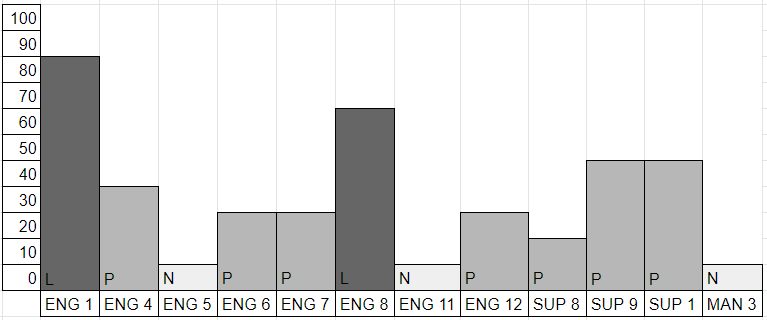
\includegraphics[scale=1]{img/ProcPries}
		\caption{PKP brandra prieš pagerinimą} % Antraštė įterpiama po paveikslėlio
		\label{img:pkpPries}
	\end{figure}

\section{Reikalavimų išsiaiškinimo (ENG 1) proceso pagerinimas}

	Buvo nuspręsta padidinti gebėjimo lygį reikalavimo išsiaiškinimo procesui, kadangi šitas procesas kompanijoje atrodo labiausiai išvystitas.
	Taip pat gebėjimas bendrauti su užsakovais ir tiksliai išsiaiškinti reikalavimus atrodo kaip labai reikalingas pradinis žingsnis kiekvienoje įmonėje.
	Visi kiti procesai gali būti tobuli, tačiau jeigu pradiniai reikalavimai būs netinkamai arba blogai užrašyti ir išsiaikinti, like procesai būs gamins tiesiog netinkamą produktą.

\subsection{Pagerinimas}

	\begin{enumerate}
		\item{Išreikštinai pridedamas bendravimas su būsimos programų sistemos vartotojais reikalavimų cikle.}
		\item{Išreikštinai surenkami parašai is galutinių vartotojų, užsakovų ir tiekėjų, kad reikalavimai buvo suprasti, kaip užrašti jie dokumente.}
		\item{Aiškiau aprašomas defekto analizės procesas.}
		\item{Pridėtas reikalavimų stebėjimo mechanizmas naudojant programinę sistemą, ne vien naudojamasi dokumentais.}
	\end{enumerate}

	\begin{figure}[htbp]
		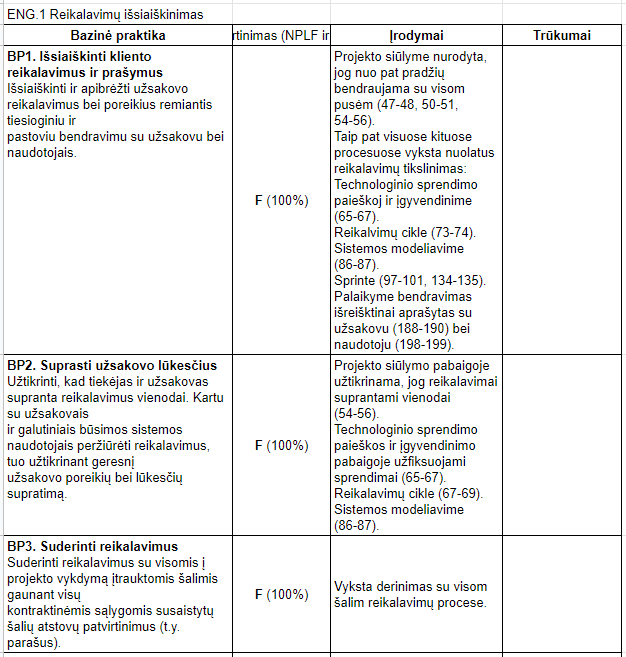
\includegraphics[scale=1]{img/eng1one}
		\caption{PKP ENG1  proceso branda po pagerinimo} % Antraštė įterpiama po paveikslėlio
		\label{img:pkpPries}
	\end{figure}

	\begin{figure}[htbp]
		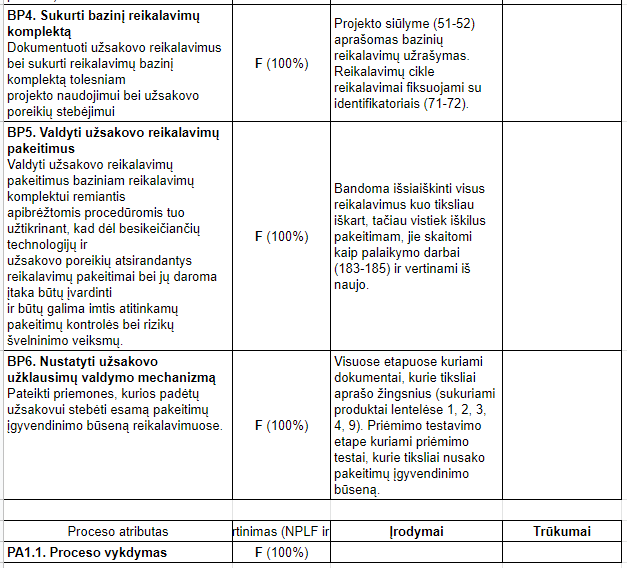
\includegraphics[scale=1]{img/eng1two}
		\caption{PKP brandra prieš pagerinimą} % Antraštė įterpiama po paveikslėlio
		\label{img:pkpPries}
	\end{figure}

\section{Programinės įrangos testavimo (ENG 8) proceso pagerinimas}	
	Kadangi labai svarbus klientų pasitikėjimas mūsų produkto kokybe, pasirinkome gerinti programinės įrangos testavimo procesą. Testuodami norime užtikrinti, kad perdavus klientui produktą neatsiras kalnas problemų ir jis veiks visose aplinkose, kuriose turi veikti.
	\subsection{Pagerinimas}
	Buvo įvesti keli pagerinimai kokybės užtikrinimo skyriuje:
	\begin{enumerate}
						\item Prie sukuriamų produktų pridedama vartotojo dokumentacija.
						\item Pridėtas pradinių duomenų apibrėžimas.
						\item Paminėta, kad sudaryti testai padengia visus su testuojama užduotim susijusius reikalavimus.
	\end{enumerate}
	Pagrinde, ką reikėjo padaryti, kad pagerinti procesą, tai papildyti ir detaliau aprašyti dokumentaciją - testai tie patys: modulių, integraciniai, automatizuojami, regresiniai testai, bet aiškiau aprašyta, kokio rezultato po testavimo tikimasi.
	\newpage
	
	\subsection{NPLF atitikimas po pagerinimo}
	\begin{figure}[htbp]
		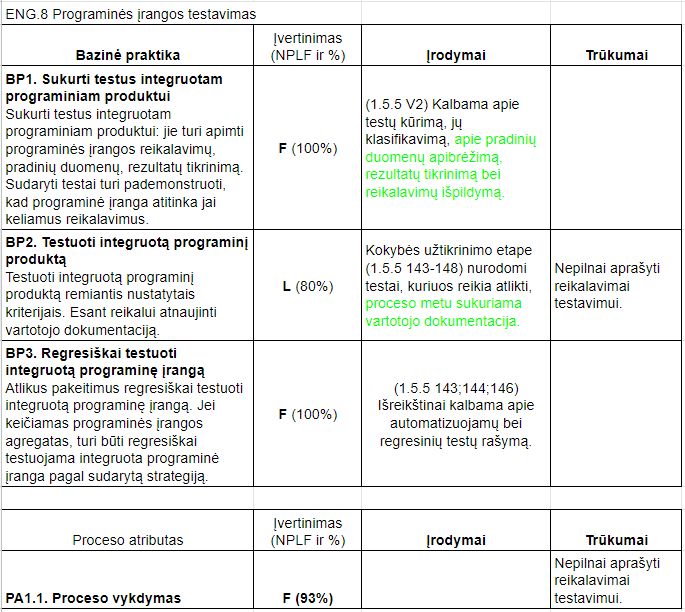
\includegraphics[scale=0.9]{img/eng8_po_pakeitimo}
		\caption{PKP ENG8 proceso branda po pagerinimo} % Antraštė įterpiama po paveikslėlio
		\label{img:pkpPries}
	\end{figure}
	
\section{Kokybės užtikrinimo (SUP 1) proceso pagerinimas}
	Pasirinkome pagerinti kokybės užtikrinimo procesą, nes manome, kad siekiant išlaikyti esamus klientus ir pritraukti ateities klientus svarbiau yra užtikrinti, 
	kad sukurtos programos būtų paprastos ir kokybiškos, negu su daug funkcionalumų, tačiau prastai veikiančios.

			\subsection{Pagerinimas}
				Įvedamos procesų gerinimo metrikos.
				Pradėjus naują projektą kiekvieno proceso metu projektų vadovas žymisi metrikas apie procesą.
					\begin{enumerate}
						\item{Proceso unikalus indikatorius (kiekvienam projektui skirtingas)}
						\item{Kokia buvo numatyta proceso trukmė}
						\item{Kiek laiko truko procesas}
						\item{Ar visos numatytos šalys dalyvavo projekte}
						\item{Kiek proceso veiklų buvo įgyvendinta}
						\item{Proceso kaina}
						\item{Atsiliepimai apie procesą}
					\end{enumerate}
				Pagal šias metrikas projekto pabaigoje, per projekto aptarimą, yra vykdomas pačio proceso aptarimas ir, jeigu to reikia, gerinimas.

				Jeigu projekto vadovas mato, kad pačio projekto vykdymo metu būtinas proceso pakeitimas, yra daromas susirinkimas su kompanijos savininkais ir suinteresuotais asmenimis siekiant spręsti šį klausimą. 
				Jeigu reikia, proceso modelio gerinimo procesas yra pradedamas anksčiau ir modelio pakeitimai yra įgyvendinami kaip galima greičiau.
\pagebreak
	\begin{center}
		\begin{table}[ht]
			\caption{Programų kūrimo proceso gerinimo procesas}
			\begin{tabular}{ | l | l | }
				\hline
				Pavadinimas:		& Proceso gerinimas.						\\ \hline
				Tikslas:		& Aptarti praėjusio projekto programų kūrimo procesą ir pagerinti jį.			\\ \hline
				Vykdytojai:		& Įmonės darbuotojai, dirbę prie projekto, ir įmonės vadovybė.					\\ \hline
				Veiklos:		& V1 - Aptariamas kiekvienas modelio procesas. 				\\
							& V2 - Apžvelgiamos metrikos.	\\
							& V3 - Surašomi gerinimo pasiūlymai.				\\ 
							& V4 - Atliekama proceso gerinimo atsiperkamumo analizė \\ 
							& V5 - Sudaromas naujas programų sistemų kūrimo modelis \\ \hline
				Naudojami produktai:	& NP1 - Proceso gerinimo metrikos. 				\\ \hline
				Sukuriami produktai:	& SP1 - Pagerintas programų kūrimo proceso modelis.		\\ \hline
			\end{tabular}
		\end{table}
	\end{center}

	\begin{enumerate}
		\item{Bendrais bruožais aptariamas kiekvienas modelio procesas, kokia komandos nuomonė, kaip sekėsi sekti proceso nurodymus jų pačių akimis ir ar procesas jiems padėjo.}
		\item{Apžvelgiamos metrikos ir kaip jos atsispindi tame, kas buvo kalbama pirmoje veikloje. 
			Išsiaiškinama, kodėl nebuvo laikomasi proceso nurodymų, kodėl jis užtruko ilgiau arba trumpiau negu planuota, ir kodėl buvo sunaudota daugiau arba mažiau pinigų negu planuota.}
		\item{Kiekvienas susirinkimo dalyvis anonimiškai surašo savo pasiūlymus, kaip gerinti procesą.
			Pasiūlymai peržiūrimi susitikimo dalyvių ir iškeliama diskusija trumpai aptariant visus nesidubliuojančius pasiūlymus.}
		\item{Pagal atrinktus pasiūlymus ir vadovybės išskirtus proceso gerinimo tikslus įvertinama, kiek kiekviena gerinimo veikla kainuos implementuoti į modelį ir koks bus trumpalaikis ir ilgalaikis veikos atsiperkamumas.}
		\item{Atmetus nereikalingus tikslus sukuriamas naujas programų sistemos kūrimos proceso modelis, kuriuo bus vadovaujamasi kituose projektuose.}
	\end{enumerate}

	Pastaba: jeigu modeliui pasikeitus projektas vis dar vyksta ir pakeitimai nėra kritiniai, liekama prie senos modelio versijos siekiant negluminti užsakovo.	

	\begin{figure}[htbp]
		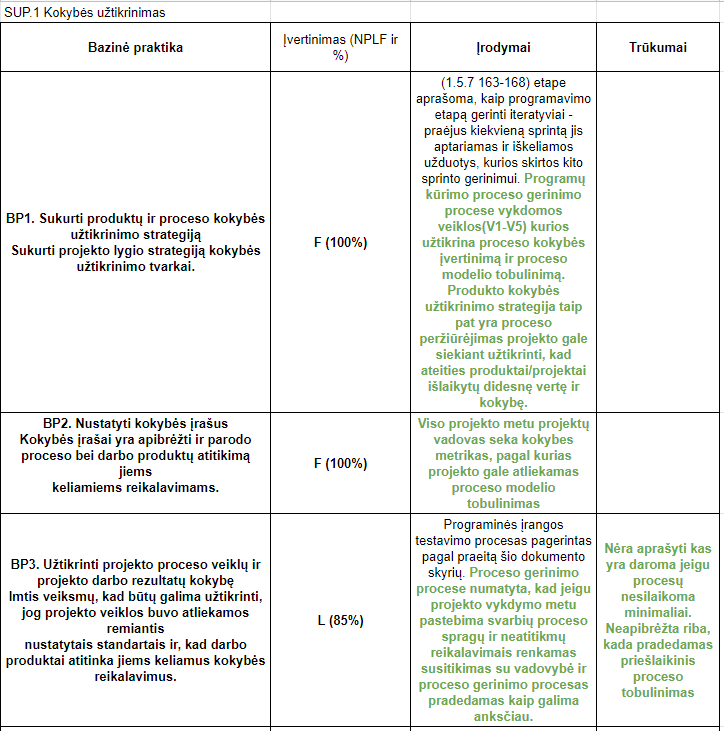
\includegraphics[scale=0.9]{img/sup1one}
		\caption{PKP SUP1 proceso branda po pagerinimo} % Antraštė įterpiama po paveikslėlio
		\label{img:pkpPries}
	\end{figure}	

	\begin{figure}[htbp]
		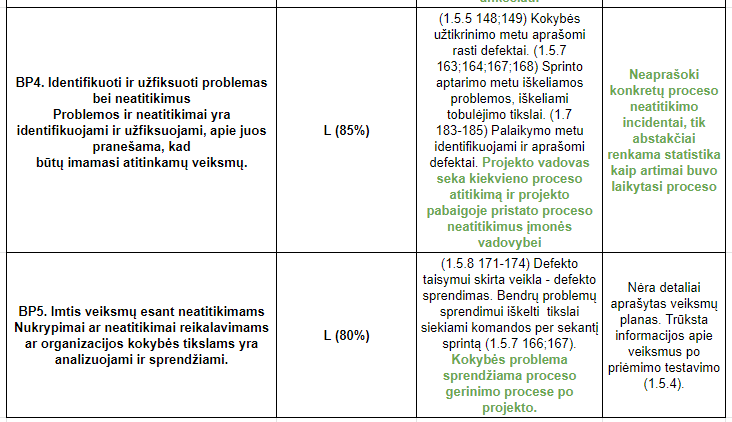
\includegraphics[scale=0.9]{img/sup1two}
		\caption{PKP SUP1 proceso branda po pagerinimo} % Antraštė įterpiama po paveikslėlio
		\label{img:pkpPries}
	\end{figure}	

	\subsection{NPLF atitikimas po pagerinimo}

	\begin{figure}[htbp]
		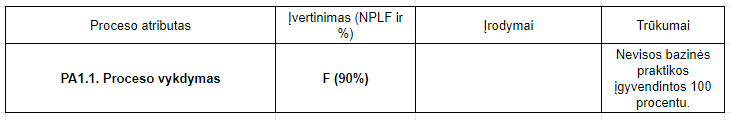
\includegraphics[scale=0.9]{img/sup1three}
		\caption{PKP SUP1 proceso branda po pagerinimo} % Antraštė įterpiama po paveikslėlio
		\label{img:pkpPries}
	\end{figure}	

\section{Rezultatai ir išvados}
	\begin{figure}[htbp]
		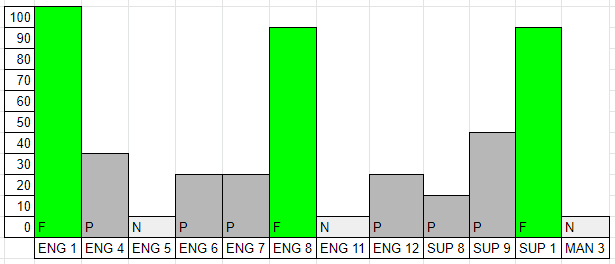
\includegraphics[scale=1]{img/ProcPo}
		\caption{Po procesų pagerinimo} % Antraštė įterpiama po paveikslėlio
		\label{img:pkpPries}
	\end{figure}

	Po procesų pagerinimo pavyko sėkmingai pakelti tris procesus iki pirmo PKP brandos lygio. 
	Išsiaiškinom ir supratom, kad net ir nedideli bet tikslingi pakeitimai procese padaro daug teigiamos įtakos kokybei. 

\end{document}
